% Options for packages loaded elsewhere
% Options for packages loaded elsewhere
\PassOptionsToPackage{unicode}{hyperref}
\PassOptionsToPackage{hyphens}{url}
%
\documentclass[
  ignorenonframetext,
  compress, aspectratio=149]{beamer}
\newif\ifbibliography
\usepackage{pgfpages}
\setbeamertemplate{caption}[numbered]
\setbeamertemplate{caption label separator}{: }
\setbeamercolor{caption name}{fg=normal text.fg}
\beamertemplatenavigationsymbolshorizontal
% remove section numbering
\setbeamertemplate{part page}{
  \centering
  \begin{beamercolorbox}[sep=16pt,center]{part title}
    \usebeamerfont{part title}\insertpart\par
  \end{beamercolorbox}
}
\setbeamertemplate{section page}{
  \centering
  \begin{beamercolorbox}[sep=12pt,center]{section title}
    \usebeamerfont{section title}\insertsection\par
  \end{beamercolorbox}
}
\setbeamertemplate{subsection page}{
  \centering
  \begin{beamercolorbox}[sep=8pt,center]{subsection title}
    \usebeamerfont{subsection title}\insertsubsection\par
  \end{beamercolorbox}
}
% Prevent slide breaks in the middle of a paragraph
\widowpenalties 1 10000
\raggedbottom
\AtBeginPart{
  \frame{\partpage}
}
\AtBeginSection{
  \ifbibliography
  \else
    \frame{\sectionpage}
  \fi
}
\AtBeginSubsection{
  \frame{\subsectionpage}
}
\usepackage{iftex}
\ifPDFTeX
  \usepackage[T1]{fontenc}
  \usepackage[utf8]{inputenc}
  \usepackage{textcomp} % provide euro and other symbols
\else % if luatex or xetex
  \usepackage{unicode-math} % this also loads fontspec
  \defaultfontfeatures{Scale=MatchLowercase}
  \defaultfontfeatures[\rmfamily]{Ligatures=TeX,Scale=1}
\fi
\usepackage{lmodern}

\usetheme[]{Montpellier}
\usecolortheme[]{dove}
\useinnertheme[]{rounded}
\useoutertheme[]{miniframes}
\ifPDFTeX\else
  % xetex/luatex font selection
\fi
% Use upquote if available, for straight quotes in verbatim environments
\IfFileExists{upquote.sty}{\usepackage{upquote}}{}
\IfFileExists{microtype.sty}{% use microtype if available
  \usepackage[]{microtype}
  \UseMicrotypeSet[protrusion]{basicmath} % disable protrusion for tt fonts
}{}
\makeatletter
\@ifundefined{KOMAClassName}{% if non-KOMA class
  \IfFileExists{parskip.sty}{%
    \usepackage{parskip}
  }{% else
    \setlength{\parindent}{0pt}
    \setlength{\parskip}{6pt plus 2pt minus 1pt}}
}{% if KOMA class
  \KOMAoptions{parskip=half}}
\makeatother

\usepackage{color}
\usepackage{fancyvrb}
\newcommand{\VerbBar}{|}
\newcommand{\VERB}{\Verb[commandchars=\\\{\}]}
\DefineVerbatimEnvironment{Highlighting}{Verbatim}{commandchars=\\\{\}}
% Add ',fontsize=\small' for more characters per line
\newenvironment{Shaded}{}{}
\newcommand{\AlertTok}[1]{\textcolor[rgb]{0.75,0.01,0.01}{\textbf{\colorbox[rgb]{0.97,0.90,0.90}{#1}}}}
\newcommand{\AnnotationTok}[1]{\textcolor[rgb]{0.79,0.38,0.79}{#1}}
\newcommand{\AttributeTok}[1]{\textcolor[rgb]{0.00,0.34,0.68}{#1}}
\newcommand{\BaseNTok}[1]{\textcolor[rgb]{0.69,0.50,0.00}{#1}}
\newcommand{\BuiltInTok}[1]{\textcolor[rgb]{0.39,0.29,0.61}{\textbf{#1}}}
\newcommand{\CharTok}[1]{\textcolor[rgb]{0.57,0.30,0.62}{#1}}
\newcommand{\CommentTok}[1]{\textcolor[rgb]{0.54,0.53,0.53}{#1}}
\newcommand{\CommentVarTok}[1]{\textcolor[rgb]{0.00,0.58,1.00}{#1}}
\newcommand{\ConstantTok}[1]{\textcolor[rgb]{0.67,0.33,0.00}{#1}}
\newcommand{\ControlFlowTok}[1]{\textcolor[rgb]{0.12,0.11,0.11}{\textbf{#1}}}
\newcommand{\DataTypeTok}[1]{\textcolor[rgb]{0.00,0.34,0.68}{#1}}
\newcommand{\DecValTok}[1]{\textcolor[rgb]{0.69,0.50,0.00}{#1}}
\newcommand{\DocumentationTok}[1]{\textcolor[rgb]{0.38,0.47,0.50}{#1}}
\newcommand{\ErrorTok}[1]{\textcolor[rgb]{0.75,0.01,0.01}{\underline{#1}}}
\newcommand{\ExtensionTok}[1]{\textcolor[rgb]{0.00,0.58,1.00}{\textbf{#1}}}
\newcommand{\FloatTok}[1]{\textcolor[rgb]{0.69,0.50,0.00}{#1}}
\newcommand{\FunctionTok}[1]{\textcolor[rgb]{0.39,0.29,0.61}{#1}}
\newcommand{\ImportTok}[1]{\textcolor[rgb]{1.00,0.33,0.00}{#1}}
\newcommand{\InformationTok}[1]{\textcolor[rgb]{0.69,0.50,0.00}{#1}}
\newcommand{\KeywordTok}[1]{\textcolor[rgb]{0.12,0.11,0.11}{\textbf{#1}}}
\newcommand{\NormalTok}[1]{\textcolor[rgb]{0.12,0.11,0.11}{#1}}
\newcommand{\OperatorTok}[1]{\textcolor[rgb]{0.79,0.38,0.79}{#1}}
\newcommand{\OtherTok}[1]{\textcolor[rgb]{0.00,0.43,0.16}{#1}}
\newcommand{\PreprocessorTok}[1]{\textcolor[rgb]{0.00,0.43,0.16}{#1}}
\newcommand{\RegionMarkerTok}[1]{\textcolor[rgb]{0.00,0.34,0.68}{\colorbox[rgb]{0.88,0.91,0.97}{#1}}}
\newcommand{\SpecialCharTok}[1]{\textcolor[rgb]{0.24,0.68,0.91}{#1}}
\newcommand{\SpecialStringTok}[1]{\textcolor[rgb]{1.00,0.33,0.00}{#1}}
\newcommand{\StringTok}[1]{\textcolor[rgb]{0.75,0.01,0.01}{#1}}
\newcommand{\VariableTok}[1]{\textcolor[rgb]{0.00,0.34,0.68}{#1}}
\newcommand{\VerbatimStringTok}[1]{\textcolor[rgb]{0.75,0.01,0.01}{#1}}
\newcommand{\WarningTok}[1]{\textcolor[rgb]{0.75,0.01,0.01}{#1}}

\usepackage{longtable,booktabs,array}
\usepackage{calc} % for calculating minipage widths
\usepackage{caption}
% Make caption package work with longtable
\makeatletter
\def\fnum@table{\tablename~\thetable}
\makeatother
\usepackage{graphicx}
\makeatletter
\newsavebox\pandoc@box
\newcommand*\pandocbounded[1]{% scales image to fit in text height/width
  \sbox\pandoc@box{#1}%
  \Gscale@div\@tempa{\textheight}{\dimexpr\ht\pandoc@box+\dp\pandoc@box\relax}%
  \Gscale@div\@tempb{\linewidth}{\wd\pandoc@box}%
  \ifdim\@tempb\p@<\@tempa\p@\let\@tempa\@tempb\fi% select the smaller of both
  \ifdim\@tempa\p@<\p@\scalebox{\@tempa}{\usebox\pandoc@box}%
  \else\usebox{\pandoc@box}%
  \fi%
}
% Set default figure placement to htbp
\def\fps@figure{htbp}
\makeatother





\setlength{\emergencystretch}{3em} % prevent overfull lines

\providecommand{\tightlist}{%
  \setlength{\itemsep}{0pt}\setlength{\parskip}{0pt}}



 


\usepackage{graphicx}
\usepackage{xcolor}
\AtBeginSubsection{}
\AtBeginDocument{\author[Ottavia M. Epifania]{Ottavia M. Epifania \\ University of Trento \\\texttt{ottavia.epifania@unitn.it}}}
\AtBeginDocument{\institute[]{A.A. 2025/2026} }
\AtBeginSection[] { \begin{frame}[plain] \tableofcontents[currentsection, hideallsubsections] \end{frame} }
\AtBeginSubsection[] { \begin{frame}[plain] \tableofcontents[currentsection,currentsubsection,hideothersubsections] \end{frame} }
\makeatletter
\@ifpackageloaded{tcolorbox}{}{\usepackage[skins,breakable]{tcolorbox}}
\@ifpackageloaded{fontawesome5}{}{\usepackage{fontawesome5}}
\definecolor{quarto-callout-color}{HTML}{909090}
\definecolor{quarto-callout-note-color}{HTML}{0758E5}
\definecolor{quarto-callout-important-color}{HTML}{CC1914}
\definecolor{quarto-callout-warning-color}{HTML}{EB9113}
\definecolor{quarto-callout-tip-color}{HTML}{00A047}
\definecolor{quarto-callout-caution-color}{HTML}{FC5300}
\definecolor{quarto-callout-color-frame}{HTML}{acacac}
\definecolor{quarto-callout-note-color-frame}{HTML}{4582ec}
\definecolor{quarto-callout-important-color-frame}{HTML}{d9534f}
\definecolor{quarto-callout-warning-color-frame}{HTML}{f0ad4e}
\definecolor{quarto-callout-tip-color-frame}{HTML}{02b875}
\definecolor{quarto-callout-caution-color-frame}{HTML}{fd7e14}
\makeatother
\makeatletter
\@ifpackageloaded{caption}{}{\usepackage{caption}}
\AtBeginDocument{%
\ifdefined\contentsname
  \renewcommand*\contentsname{Table of contents}
\else
  \newcommand\contentsname{Table of contents}
\fi
\ifdefined\listfigurename
  \renewcommand*\listfigurename{List of Figures}
\else
  \newcommand\listfigurename{List of Figures}
\fi
\ifdefined\listtablename
  \renewcommand*\listtablename{List of Tables}
\else
  \newcommand\listtablename{List of Tables}
\fi
\ifdefined\figurename
  \renewcommand*\figurename{Figure}
\else
  \newcommand\figurename{Figure}
\fi
\ifdefined\tablename
  \renewcommand*\tablename{Table}
\else
  \newcommand\tablename{Table}
\fi
}
\@ifpackageloaded{float}{}{\usepackage{float}}
\floatstyle{ruled}
\@ifundefined{c@chapter}{\newfloat{codelisting}{h}{lop}}{\newfloat{codelisting}{h}{lop}[chapter]}
\floatname{codelisting}{Listing}
\newcommand*\listoflistings{\listof{codelisting}{List of Listings}}
\makeatother
\makeatletter
\makeatother
\makeatletter
\@ifpackageloaded{caption}{}{\usepackage{caption}}
\@ifpackageloaded{subcaption}{}{\usepackage{subcaption}}
\makeatother

\usepackage{bookmark}
\IfFileExists{xurl.sty}{\usepackage{xurl}}{} % add URL line breaks if available
\urlstyle{same}
\hypersetup{
  pdftitle={Modulo Didattico 1: Introduzione a R},
  pdfauthor={Ottavia M. Epifania},
  hidelinks,
  pdfcreator={LaTeX via pandoc}}


\title{Modulo Didattico 1: Introduzione a \texttt{R}}
\subtitle{Corso Analisi dei dati con applicazioni informatiche}
\author{Ottavia M. Epifania}
\date{}

\begin{document}
\frame{\titlepage}


\section{Il corso}\label{il-corso}

\begin{frame}{}
\phantomsection\label{section}
Lezioni:

\begin{itemize}
\tightlist
\item
  Martedì: 10:30-12:30 (orario reale: 10:30 - 12:00)
\item
  Giovedì: 13:00-15:00 (orario reale: 13:30 - 15:00)
\item
  Venerdì: 10:30-12:30 (orario reale: 10:30 - 12:00)
\end{itemize}

Ricevimento: su appuntamento, prevalentemente online

\begin{center}
ottavia.epifania@unitn.it
\end{center}
\end{frame}

\section{Introduzione}\label{introduzione}

\subsection{Evoluzione e storia di R}\label{evoluzione-e-storia-di-r}

\begin{frame}{}
\phantomsection\label{section-1}
\begin{itemize}
\tightlist
\item
  Discende da S e S+
\item
  Parte del progetto GNU
\item
  Software libero sotto licenza GNU GPL
\item
  Open Source
\item
  \url{https://www.r-project.org/COPYING}
\end{itemize}
\end{frame}

\subsection{Caratteristiche di R}\label{caratteristiche-di-r}

\begin{frame}{}
\phantomsection\label{section-2}
\begin{tcolorbox}[enhanced jigsaw, rightrule=.15mm, titlerule=0mm, colbacktitle=quarto-callout-tip-color!10!white, left=2mm, title={Pros}, coltitle=black, leftrule=.75mm, arc=.35mm, opacityback=0, bottomtitle=1mm, breakable, toprule=.15mm, colback=white, colframe=quarto-callout-tip-color-frame, toptitle=1mm, opacitybacktitle=0.6, bottomrule=.15mm]

Linguaggio object-oriented

Più dimestichezza nell'analisi dei dati, più conoscenza del dato,
modelli più complessi

Permette di addentrarsi sempre di più nei linguaggi di programmazione

\end{tcolorbox}

\begin{tcolorbox}[enhanced jigsaw, rightrule=.15mm, titlerule=0mm, colbacktitle=quarto-callout-warning-color!10!white, left=2mm, title={Cons}, coltitle=black, leftrule=.75mm, arc=.35mm, opacityback=0, bottomtitle=1mm, breakable, toprule=.15mm, colback=white, colframe=quarto-callout-warning-color-frame, toptitle=1mm, opacitybacktitle=0.6, bottomrule=.15mm]

Difficile da imparare (all'inizio)

Non è intuitivo (all'inizio) \(\rightarrow\) se non si ha già una vaga
idea di dove partire non si riesce a fare nulla

\end{tcolorbox}
\end{frame}

\section{RStudio}\label{rstudio}

\begin{frame}{}
\phantomsection\label{section-3}
\vspace*{-0.5mm}

\begin{center}

\includegraphics[width=1.1\linewidth,height=\textheight,keepaspectratio]{img/Rstudio.png}
\end{center}
\end{frame}

\begin{frame}[fragile]{console vs.~script}
\phantomsection\label{console-vs.-script}
\begin{tcolorbox}[enhanced jigsaw, rightrule=.15mm, titlerule=0mm, colbacktitle=quarto-callout-note-color!10!white, left=2mm, title={Console}, coltitle=black, leftrule=.75mm, arc=.35mm, opacityback=0, bottomtitle=1mm, breakable, toprule=.15mm, colback=white, colframe=quarto-callout-note-color-frame, toptitle=1mm, opacitybacktitle=0.6, bottomrule=.15mm]

I comandi nella console vengono eseguiti e non salvati

Per eseguire il comando \(\rightarrow\) \texttt{Invio}

L'output è immediato ed appare nella console

\end{tcolorbox}

\pause

\begin{tcolorbox}[enhanced jigsaw, rightrule=.15mm, titlerule=0mm, colbacktitle=quarto-callout-note-color!10!white, left=2mm, title={Script}, coltitle=black, leftrule=.75mm, arc=.35mm, opacityback=0, bottomtitle=1mm, breakable, toprule=.15mm, colback=white, colframe=quarto-callout-note-color-frame, toptitle=1mm, opacitybacktitle=0.6, bottomrule=.15mm]

è possibile salvare gli script con tutti i comandi salvati

Per eseguire il comando \(\rightarrow\) \texttt{Ctrl\ +\ Invio}
(\texttt{cmd\ +\ Enter})

L'output è restituito nella console

\end{tcolorbox}

\small

Per passare alla console \(\rightarrow\) \texttt{ctrl\ +\ 2}

Per passare allo script \(\rightarrow\) \texttt{ctr\ +\ 1}
\end{frame}

\section{Operatori}\label{operatori}

\subsection{Matematici}\label{matematici}

\begin{frame}[fragile]{}
\phantomsection\label{section-4}
\begin{longtable}[]{@{}ll@{}}
\toprule\noalign{}
Simbolo & Significato \\
\midrule\noalign{}
\endhead
+ & Addizione \\
- & Sottrazione \\
* & Moltiplicazione \\
/ & Divisione \\
\^{} & Potenza \\
\bottomrule\noalign{}
\end{longtable}

\textbf{Esempio}:

\begin{Shaded}
\begin{Highlighting}[]
\NormalTok{(((}\DecValTok{4} \SpecialCharTok{*} \DecValTok{2}\NormalTok{) }\SpecialCharTok{{-}} \DecValTok{7}\NormalTok{) }\SpecialCharTok{+} \DecValTok{2}\NormalTok{)}\SpecialCharTok{\^{}}\DecValTok{3}
\end{Highlighting}
\end{Shaded}

\pause

\begin{verbatim}
[1] 27
\end{verbatim}
\end{frame}

\begin{frame}[fragile]{}
\phantomsection\label{section-5}
\begin{longtable}[]{@{}ll@{}}
\toprule\noalign{}
Simbolo & Significato \\
\midrule\noalign{}
\endhead
\textless{} & Minore \\
\textgreater{} & Maggiore \\
\textless= & Minore o uguale \\
\textgreater= & Maggiore o uguale \\
== & Uguale \\
!= & Diverso \\
\bottomrule\noalign{}
\end{longtable}

\small

\textbf{Esempio}:

\begin{Shaded}
\begin{Highlighting}[]
\NormalTok{(}\DecValTok{10} \SpecialCharTok{/} \DecValTok{2}\NormalTok{) }\SpecialCharTok{\textgreater{}} \DecValTok{3}
\end{Highlighting}
\end{Shaded}

\begin{verbatim}
[1] TRUE
\end{verbatim}
\end{frame}

\subsection{Insiemistici}\label{insiemistici}

\begin{frame}[fragile]{}
\phantomsection\label{section-6}
\begin{longtable}[]{@{}ll@{}}
\toprule\noalign{}
Simbolo & Significato \\
\midrule\noalign{}
\endhead
\texttt{\&} & AND (congiunzione \(\land\)) \\
& \\
\texttt{!} & NOT (negazione \(\lnot\)) \\
\texttt{\textbar{}} & OR (Disgiunzione \(\lor\)) \\
\bottomrule\noalign{}
\end{longtable}

\textbf{Esempio}:

\begin{Shaded}
\begin{Highlighting}[]
\NormalTok{(}\DecValTok{2} \SpecialCharTok{\textgreater{}} \DecValTok{3}\NormalTok{) }\SpecialCharTok{\&}\NormalTok{ (}\DecValTok{5} \SpecialCharTok{\textless{}} \DecValTok{10}\NormalTok{)}
\end{Highlighting}
\end{Shaded}

\pause

\begin{verbatim}
[1] FALSE
\end{verbatim}
\end{frame}

\subsection{Tavole di verità}\label{tavole-di-verituxe0}

\begin{frame}{}
\phantomsection\label{section-7}
\begin{table}

\caption{\label{tbl-tables}Tavole di verità}

\begin{minipage}{0.50\linewidth}

\subcaption{\label{tbl-tables-1}Congiunzione}

\centering{

\begin{tabular}{lll}
\toprule
\(a\) & \(b\) & \(a \land b\)\\
\midrule
V & V & V\\
V & F & F\\
F & V & F\\
F & F & F\\
\bottomrule
\end{tabular}

}

\end{minipage}%
%
\begin{minipage}{0.50\linewidth}

\subcaption{\label{tbl-tables-2}Disgiunzione}

\centering{

\begin{tabular}{lll}
\toprule
\(a\) & \(b\) & \(a \lor b\)\\
\midrule
V & V & V\\
V & F & V\\
F & V & V\\
F & F & F\\
\bottomrule
\end{tabular}

}

\end{minipage}%
\newline
\begin{minipage}{0.50\linewidth}

\subcaption{\label{tbl-tables-3}Negazione}

\centering{

\begin{tabular}{ll}
\toprule
\(a\) & \(\lnot a\)\\
\midrule
V & F\\
F & V\\
\bottomrule
\end{tabular}

}

\end{minipage}%

\end{table}%
\end{frame}

\subsection{Funzioni matematiche di
base}\label{funzioni-matematiche-di-base}

\begin{frame}[fragile]{}
\phantomsection\label{section-8}
\begin{longtable}[]{@{}ll@{}}
\toprule\noalign{}
Funzione & Significato \\
\midrule\noalign{}
\endhead
\texttt{log()} & Logaritmo naturale \\
\texttt{exp()} & Esponenziale \\
\texttt{abs()} & Valore assoluto \\
\texttt{sqrt()} & Radice quadrata \\
\texttt{round()} & Arrotondamento \\
\texttt{mean()} & Media \\
\texttt{min()}, \texttt{max()} & Minimo, Massimo \\
\texttt{sd()}, \texttt{var()} & Deviazione st., Varianza \\
\texttt{sum()} & Somma \\
\bottomrule\noalign{}
\end{longtable}

\textbf{Esempio}:

\begin{Shaded}
\begin{Highlighting}[]
\FunctionTok{abs}\NormalTok{(}\FunctionTok{round}\NormalTok{(}\SpecialCharTok{{-}}\DecValTok{1} \SpecialCharTok{*}\NormalTok{ (}\DecValTok{10} \SpecialCharTok{/} \DecValTok{3}\NormalTok{), }\DecValTok{2}\NormalTok{))}
\end{Highlighting}
\end{Shaded}

\begin{verbatim}
[1] 3.33
\end{verbatim}
\end{frame}

\section{Oggetti}\label{oggetti}

\subsection{Variabili, costanti, assegnazione in
R}\label{variabili-costanti-assegnazione-in-r}

\begin{frame}[fragile]{Assegnazione e concatenazione}
\phantomsection\label{assegnazione-e-concatenazione}
\begin{itemize}
\tightlist
\item
  Assegnazione: \texttt{\textless{}-} oppure \texttt{=}
\item
  Concatenazione: \texttt{c()} serve per creare vettori di valori
\end{itemize}

\begin{Shaded}
\begin{Highlighting}[]
\FunctionTok{c}\NormalTok{(}\DecValTok{1}\NormalTok{, }\DecValTok{2}\NormalTok{, }\DecValTok{25}\NormalTok{, }\DecValTok{10}\NormalTok{)}
\end{Highlighting}
\end{Shaded}

\begin{verbatim}
[1]  1  2 25 10
\end{verbatim}

\pause

\begin{itemize}
\tightlist
\item
  Esempi di variabili: \texttt{A}, \texttt{a}, \texttt{Giorgio},
  \texttt{X3}
\item
  Costanti:

  \begin{itemize}
  \tightlist
  \item
    \texttt{pi} (3.14\ldots)
  \item
    \texttt{TRUE}, \texttt{FALSE}
  \end{itemize}
\end{itemize}
\end{frame}

\begin{frame}[fragile]{}
\phantomsection\label{section-9}
\begin{Shaded}
\begin{Highlighting}[]
\NormalTok{A }\OtherTok{\textless{}{-}} \DecValTok{12}
\NormalTok{a }\OtherTok{=} \DecValTok{6}
\NormalTok{(A }\SpecialCharTok{/}\NormalTok{ a }\SpecialCharTok{\textgreater{}} \DecValTok{0}\NormalTok{) }\SpecialCharTok{!=} \ConstantTok{TRUE}
\end{Highlighting}
\end{Shaded}

\begin{verbatim}
[1] FALSE
\end{verbatim}

\pause

\begin{Shaded}
\begin{Highlighting}[]
\NormalTok{A }\OtherTok{\textless{}{-}} \FloatTok{12.8} \CommentTok{\# variabile numerica}
\NormalTok{nome }\OtherTok{\textless{}{-}} \StringTok{"giorgio"}  \CommentTok{\# variabile character}
\NormalTok{b1 }\OtherTok{\textless{}{-}} \FunctionTok{c}\NormalTok{(}\DecValTok{12}\NormalTok{, }\FloatTok{0.3}\NormalTok{, }\DecValTok{5}\NormalTok{, }\FloatTok{778.3}\NormalTok{) }\CommentTok{\# vettore numerico}
\NormalTok{Nomi3 }\OtherTok{\textless{}{-}} \FunctionTok{c}\NormalTok{(}\StringTok{"giorgio"}\NormalTok{, }\StringTok{"ugo"}\NormalTok{, }\StringTok{"anna"}\NormalTok{) }\CommentTok{\# vettore character}
\end{Highlighting}
\end{Shaded}
\end{frame}

\subsection{Matrici}\label{matrici}

\begin{frame}[fragile]{}
\phantomsection\label{section-10}
Sono dei vettori concatenati di dimensione \(r\) (righe) \(\times c\)
(colonne)

\begin{verbatim}
  matrix(data, nrow, ncol, byrow = FALSE)
\end{verbatim}

\pause

\textbf{Creazione matrice:}

\begin{Shaded}
\begin{Highlighting}[]
\NormalTok{A }\OtherTok{\textless{}{-}} \FunctionTok{c}\NormalTok{(}\DecValTok{1}\NormalTok{, }\DecValTok{8}\NormalTok{, }\DecValTok{5}\NormalTok{, }\DecValTok{0}\NormalTok{)}
\NormalTok{M }\OtherTok{\textless{}{-}} \FunctionTok{matrix}\NormalTok{(A, }\DecValTok{2}\NormalTok{, }\DecValTok{2}\NormalTok{)}
\NormalTok{M}
\end{Highlighting}
\end{Shaded}

\begin{verbatim}
     [,1] [,2]
[1,]    1    5
[2,]    8    0
\end{verbatim}

\pause

\footnotesize

\begin{Shaded}
\begin{Highlighting}[]
\NormalTok{?matrix  }\CommentTok{\# Accede alla documentazione della funzione}
\end{Highlighting}
\end{Shaded}
\end{frame}

\begin{frame}[fragile]{Esercizio}
\phantomsection\label{esercizio}
\begin{itemize}
\tightlist
\item
  Scaricare il file \texttt{LaboratorioRmod1\_Esercizi.pdf} dalla
  piattaforma Moodle del corso
\item
  Il file contiene la traccia degli esercizi
\end{itemize}
\end{frame}

\subsection{Indicizzare e selezionare}\label{indicizzare-e-selezionare}

\begin{frame}[fragile]{Indicizzare e selezionare}
\begin{verbatim}
vettore[i],     matrice[r, c]
\end{verbatim}

\texttt{{[}i{]}}: l'indice (la posizione) dell'oggetto che si vuole
selezionare

\texttt{{[}r,\ c{]}}: riga, colonna (restituisce la cella specifica
della matrice)

\begin{columns}[T]
\begin{column}{0.5\linewidth}
\small

\begin{Shaded}
\begin{Highlighting}[]
\NormalTok{peso }\OtherTok{=} \FunctionTok{c}\NormalTok{(}\FloatTok{3.3}\NormalTok{, }\DecValTok{4}\NormalTok{, }\DecValTok{5}\NormalTok{, }\FloatTok{6.4}\NormalTok{, }\FloatTok{3.5}\NormalTok{, }\FloatTok{4.2}\NormalTok{)}
\NormalTok{peso[}\DecValTok{3}\NormalTok{]}
\end{Highlighting}
\end{Shaded}

\begin{verbatim}
[1] 5
\end{verbatim}

\begin{Shaded}
\begin{Highlighting}[]
\NormalTok{matrice }\OtherTok{=} \FunctionTok{matrix}\NormalTok{(peso, }\AttributeTok{nrow =} \DecValTok{2}\NormalTok{)}
\NormalTok{matrice}
\end{Highlighting}
\end{Shaded}

\begin{verbatim}
     [,1] [,2] [,3]
[1,]  3.3  5.0  3.5
[2,]  4.0  6.4  4.2
\end{verbatim}
\end{column}

\begin{column}{0.5\linewidth}
\small

\begin{Shaded}
\begin{Highlighting}[]
\NormalTok{matrice[}\DecValTok{1}\NormalTok{,]}
\end{Highlighting}
\end{Shaded}

\begin{verbatim}
[1] 3.3 5.0 3.5
\end{verbatim}

\begin{Shaded}
\begin{Highlighting}[]
\NormalTok{matrice[, }\DecValTok{2}\NormalTok{]}
\end{Highlighting}
\end{Shaded}

\begin{verbatim}
[1] 5.0 6.4
\end{verbatim}

\begin{Shaded}
\begin{Highlighting}[]
\NormalTok{matrice[}\DecValTok{2}\NormalTok{,}\DecValTok{2}\NormalTok{]}
\end{Highlighting}
\end{Shaded}

\begin{verbatim}
[1] 6.4
\end{verbatim}
\end{column}
\end{columns}
\end{frame}

\subsection{Dataframe}\label{dataframe}

\begin{frame}[fragile]{}
\phantomsection\label{section-11}
\begin{verbatim}
data.frame(. . .)
\end{verbatim}

Una matrice con \(r\) righe e \(c\) colonne

Può contenere variabili di tipo diverso

\small

\begin{Shaded}
\begin{Highlighting}[]
\NormalTok{sesso }\OtherTok{=} \FunctionTok{c}\NormalTok{(}\FunctionTok{rep}\NormalTok{(}\FunctionTok{c}\NormalTok{(}\StringTok{"M"}\NormalTok{,}\StringTok{"F"}\NormalTok{), }\AttributeTok{length=}\FunctionTok{length}\NormalTok{(peso)))}
\NormalTok{data }\OtherTok{=} \FunctionTok{data.frame}\NormalTok{(peso, sesso)}
\NormalTok{data}
\end{Highlighting}
\end{Shaded}

\begin{verbatim}
  peso sesso
1  3.3     M
2  4.0     F
3  5.0     M
4  6.4     F
5  3.5     M
6  4.2     F
\end{verbatim}
\end{frame}

\begin{frame}[fragile]{}
\phantomsection\label{section-12}
\begin{verbatim}
data[r, c], data$nome_variabile
\end{verbatim}

\pause

\begin{columns}[T]
\begin{column}{0.5\linewidth}
\small

\begin{Shaded}
\begin{Highlighting}[]
\NormalTok{data}
\end{Highlighting}
\end{Shaded}

\begin{verbatim}
  peso sesso
1  3.3     M
2  4.0     F
3  5.0     M
4  6.4     F
5  3.5     M
6  4.2     F
\end{verbatim}
\end{column}

\begin{column}{0.5\linewidth}
\small

\begin{Shaded}
\begin{Highlighting}[]
\NormalTok{data[}\DecValTok{2}\NormalTok{, }\DecValTok{1}\NormalTok{]}
\end{Highlighting}
\end{Shaded}

\begin{verbatim}
[1] 4
\end{verbatim}

\begin{Shaded}
\begin{Highlighting}[]
\NormalTok{data}\SpecialCharTok{$}\NormalTok{peso}
\end{Highlighting}
\end{Shaded}

\begin{verbatim}
[1] 3.3 4.0 5.0 6.4 3.5 4.2
\end{verbatim}

\begin{Shaded}
\begin{Highlighting}[]
\NormalTok{data}\SpecialCharTok{$}\NormalTok{peso[}\DecValTok{2}\NormalTok{]}
\end{Highlighting}
\end{Shaded}

\begin{verbatim}
[1] 4
\end{verbatim}
\end{column}
\end{columns}
\end{frame}

\subsection{Liste}\label{liste}

\begin{frame}[fragile]{}
\phantomsection\label{section-13}
\begin{verbatim}
  list(name1 = obj1, name2 = obj2, name3 = obj3, . . .)
  
\end{verbatim}

\small

Permette di creare liste di oggetti diversi (matrici, vettori, variabli)
di diverso tipo (\texttt{numeric}, \texttt{character}, \texttt{integer})

\pause

\footnotesize

\begin{Shaded}
\begin{Highlighting}[]
\NormalTok{A }\OtherTok{\textless{}{-}} \FunctionTok{c}\NormalTok{(}\DecValTok{1}\NormalTok{,}\DecValTok{8}\NormalTok{,}\DecValTok{5}\NormalTok{,}\DecValTok{0}\NormalTok{)}
\NormalTok{M }\OtherTok{\textless{}{-}} \FunctionTok{matrix}\NormalTok{(A, }\DecValTok{2}\NormalTok{, }\DecValTok{2}\NormalTok{)}
\NormalTok{Nomi3 }\OtherTok{\textless{}{-}} \FunctionTok{c}\NormalTok{(}\StringTok{"giorgio"}\NormalTok{, }\StringTok{"ugo"}\NormalTok{, }\StringTok{"anna"}\NormalTok{)}
\NormalTok{LV }\OtherTok{\textless{}{-}} \FunctionTok{c}\NormalTok{(}\ConstantTok{TRUE}\NormalTok{, }\ConstantTok{FALSE}\NormalTok{, }\ConstantTok{TRUE}\NormalTok{, }\ConstantTok{TRUE}\NormalTok{)}
\NormalTok{OgLista }\OtherTok{\textless{}{-}} \FunctionTok{list}\NormalTok{(}\AttributeTok{a =}\NormalTok{ A, }\AttributeTok{Mat =}\NormalTok{ M, }\AttributeTok{nomi =}\NormalTok{ Nomi3, }\AttributeTok{X =}\NormalTok{ LV)}
\FunctionTok{str}\NormalTok{(OgLista)}
\end{Highlighting}
\end{Shaded}

\begin{verbatim}
List of 4
 $ a   : num [1:4] 1 8 5 0
 $ Mat : num [1:2, 1:2] 1 8 5 0
 $ nomi: chr [1:3] "giorgio" "ugo" "anna"
 $ X   : logi [1:4] TRUE FALSE TRUE TRUE
\end{verbatim}
\end{frame}

\begin{frame}[fragile]{}
\phantomsection\label{section-14}
\begin{verbatim}
lista[[i]], lista$nome_oggettpo
\end{verbatim}

\texttt{{[}{[}i{]}{]}}: indice dell'oggetto all'interno della lista a
cui si vuole accedere

\small

\begin{Shaded}
\begin{Highlighting}[]
\NormalTok{OgLista[[}\DecValTok{2}\NormalTok{]]}
\end{Highlighting}
\end{Shaded}

\begin{verbatim}
     [,1] [,2]
[1,]    1    5
[2,]    8    0
\end{verbatim}

\texttt{\$nome\_oggetto}

\begin{Shaded}
\begin{Highlighting}[]
\NormalTok{OgLista}\SpecialCharTok{$}\NormalTok{Mat}
\end{Highlighting}
\end{Shaded}

\begin{verbatim}
     [,1] [,2]
[1,]    1    5
[2,]    8    0
\end{verbatim}
\end{frame}

\section{Importare dati esterni}\label{importare-dati-esterni}

\subsection{Importa base}\label{importa-base}

\begin{frame}[fragile]{}
\phantomsection\label{section-15}
\begin{verbatim}
read.csv2("file_path", header = T, sep = ";")
\end{verbatim}

Il default della funzione prvede che la prima riga contenga i nomi delle
variabili e che il separatore di colonne sia ``;''.

Se si possiede un dataset chiamato ``dati'' nella cartella ``data'',
questo codice lo importerà all'interno dell'ambiente

\begin{Shaded}
\begin{Highlighting}[]
\CommentTok{\# Lettura file dati esterni}
\NormalTok{data }\OtherTok{\textless{}{-}} \FunctionTok{read.csv2}\NormalTok{(}\StringTok{"data/dati.csv"}\NormalTok{)}
\end{Highlighting}
\end{Shaded}
\end{frame}

\subsection{Importa alternativa 1}\label{importa-alternativa-1}

\begin{frame}{}
\phantomsection\label{section-16}
\begin{center}
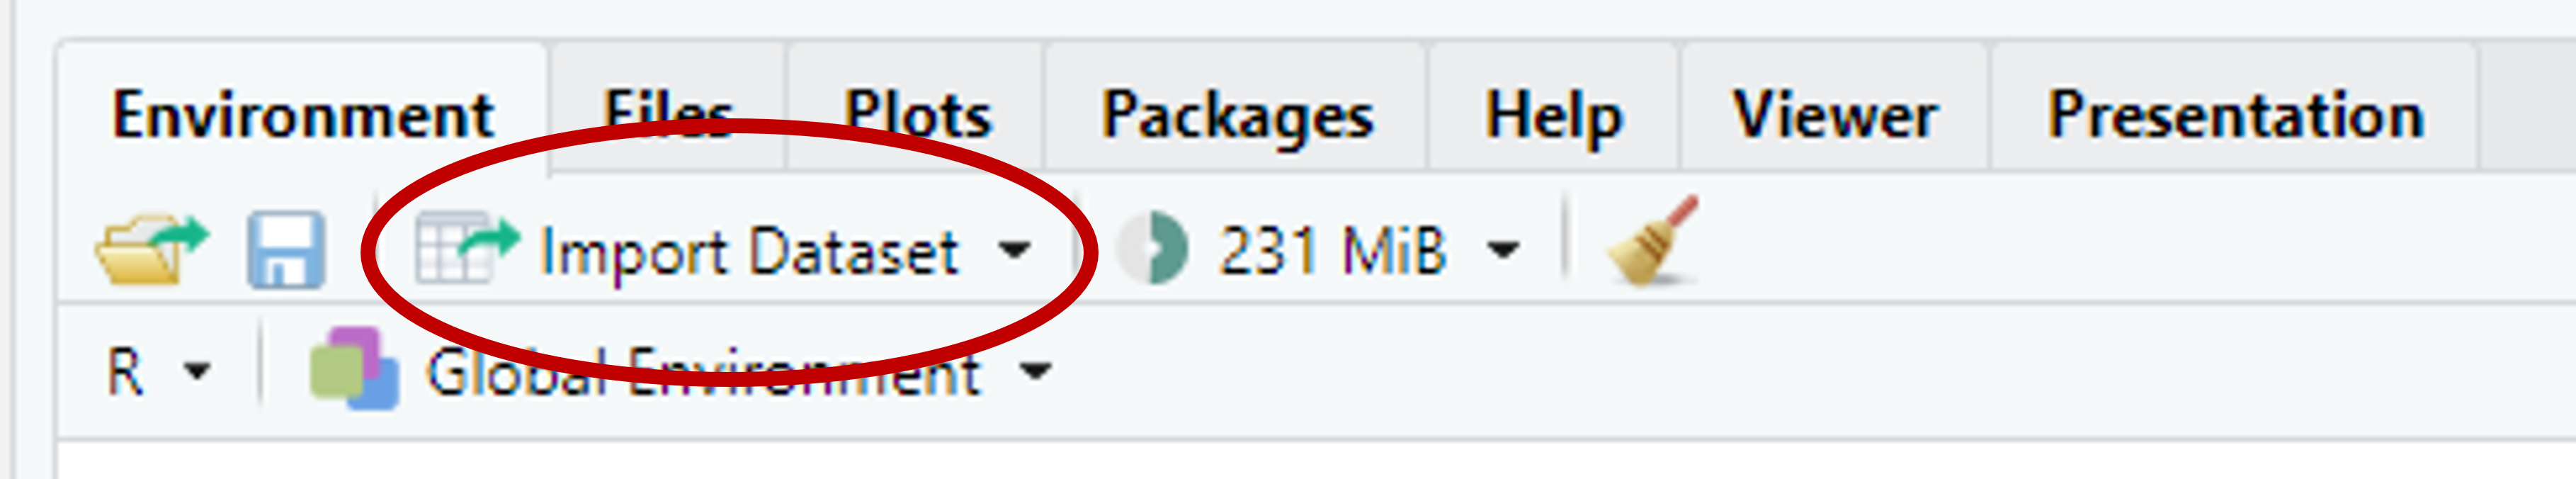
\includegraphics[width=1\linewidth,height=\textheight,keepaspectratio]{img/import0.png}
\end{center}
\end{frame}

\begin{frame}{}
\phantomsection\label{section-17}
\begin{center}
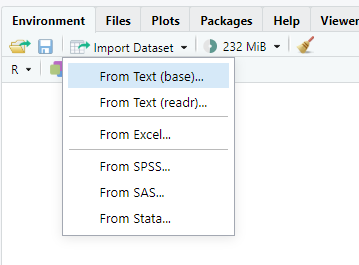
\includegraphics[width=1\linewidth,height=\textheight,keepaspectratio]{img/import1.png}
\end{center}
\end{frame}

\begin{frame}{}
\phantomsection\label{section-18}
\begin{center}
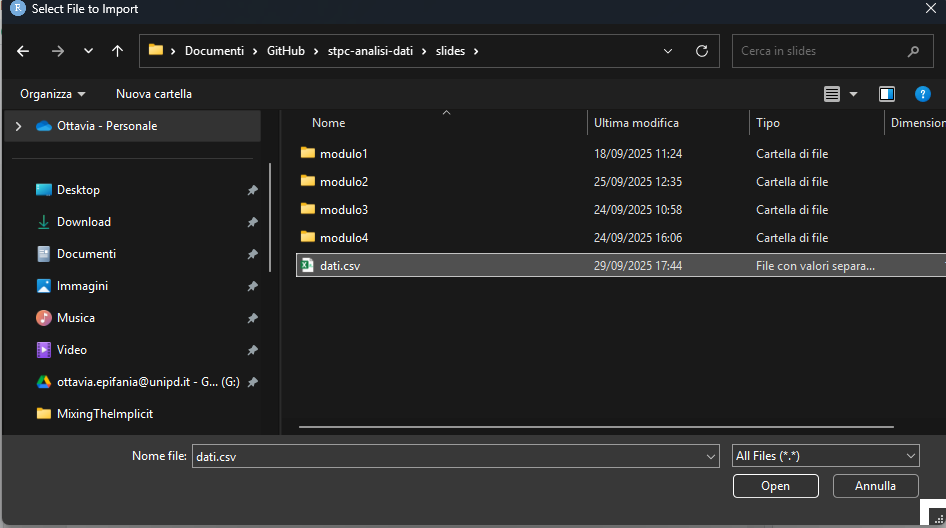
\includegraphics[width=1\linewidth,height=\textheight,keepaspectratio]{img/import2.png}
\end{center}
\end{frame}

\begin{frame}{}
\phantomsection\label{section-19}
\begin{center}
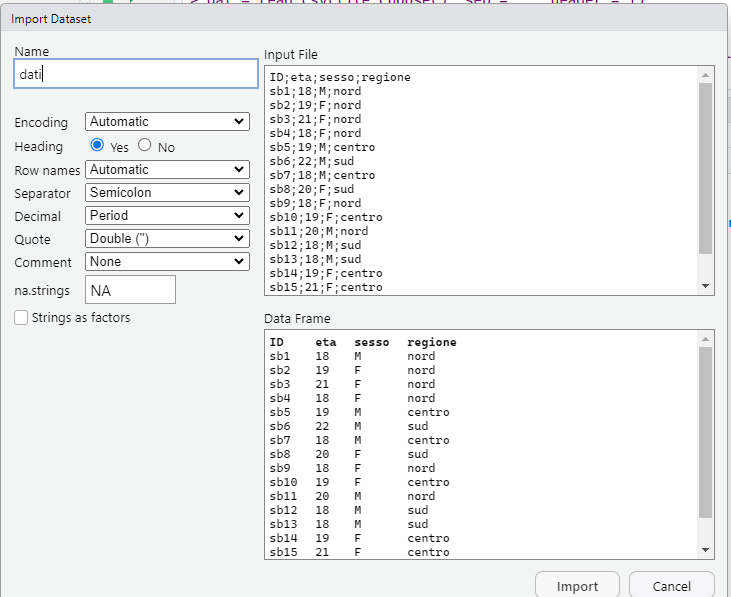
\includegraphics[width=1\linewidth,height=\textheight,keepaspectratio]{img/import3.png}
\end{center}
\end{frame}

\subsection{Importa alternativa 2}\label{importa-alternativa-2}

\begin{frame}[fragile]{}
\phantomsection\label{section-20}
\begin{Shaded}
\begin{Highlighting}[]
\NormalTok{dati }\OtherTok{=} \FunctionTok{read.csv}\NormalTok{(}\StringTok{"C:/Users/Ottavia/Documents/GitHub/stpc{-}analisi{-}dati/slides/dati.csv"}\NormalTok{, }
                \AttributeTok{sep =}\StringTok{";"}\NormalTok{, }\AttributeTok{dec =}\StringTok{","}\NormalTok{, }\AttributeTok{header =} \ConstantTok{TRUE}\NormalTok{)}
\FunctionTok{head}\NormalTok{(dati)}
\end{Highlighting}
\end{Shaded}

\begin{verbatim}
   ID eta sesso regione
1 sb1  18     M    nord
2 sb2  19     F    nord
3 sb3  21     F    nord
4 sb4  18     F    nord
5 sb5  19     M  centro
6 sb6  22     M     sud
\end{verbatim}
\end{frame}

\begin{frame}{}
\phantomsection\label{section-21}
\end{frame}




\end{document}
